\chapter{Container-Technologien}

Dieses Kapitel beschreibt mit der Betriebssystemvirtualisierung in Containern eine effektive Möglichkeit, Microservices mit allen Abhängigkeiten in eine Einheit zu verpacken und effizient zu betreiben. Die technischen Grundlagen und Voraussetzungen dafür existieren schon einige Jahre, doch erst eine Implementierung mit dem Namen \textit{Docker} brachte neuen Aufschwung in diese Art der Virtualisierung. Mittlerweile ist Docker eine allgegenwärtige Methode, Software aller Art zu verteilen und zu betreiben.

Eine Microservices"=Architektur ist nicht nur aus Softwareentwicklungssicht herausfordernd, sondern auch aus Infrastruktursicht. Jeder Microservice muss unabhängig ausgerollt und skaliert werden können. Nur so kann diese Architektur auch die in Abschnitt \ref{sec:ms-advantages} beschriebenen Vorteile entfalten. Im Unterschied zu Hardwarevirtualisierung bietet dieser Ansatz wesentlich kürzere Bereitstellungszeiten und eine effektivere Nutzung von Ressourcen.

Jeder Service hat bestimmte Voraussetzungen an seine Infrastrukturumgebung. Dazu zählen externe Bibliotheken, Konfigurationen und meistens eine Laufzeitumgebung, wie \zB Java, .NET oder Python. Nun gibt es drei Möglichkeiten, die Infrastruktur über den gesamten Lebenszyklus eines Services zu verwalten. Am schlechtesten ist die benötigte Konfiguration manuell vorzunehmen. Dadurch ist es schwierig Änderungen nachzuvollziehen und zu testen. Besser ist es die Abhängigkeiten auf einem Server mit \textit{Infrastructure-as-Code} zu installieren und laufend zu aktualisieren. Ein alternativer Ansatz ist, den Service mit seinen Abhängigkeiten und Konfigurationen in ein Betriebssystemabbild -- \textit{engl. Image} -- zu verpacken \cite[113]{newman2015building}. Anstelle einer ausführbaren Anwendung, wird einfach ein vollständiges Abbild eines virtuellen Servers erstellt und verteilt. Im folgenden Abschnitt wird dieser Ansatz noch näher präzisiert und anschließend mit Docker eine Technologie vorgestellt, die genau auf dieser Idee aufsetzt.
\section{Unveränderbarer Server}

Anstatt die Konfiguration eines Servers zu ändern, kann man ihn auch stoppen und einen neuen Server mit aktualisierter Konfiguration wieder starten. Was sich anfänglich sehr aufwändig und unsinnig anhört, ist heute aus gutem Grund gängige Praxis. Das Unternehmen Netflix beispielsweise, praktizierte diesen Ansatz bereits sehr früh \cite{NflxLegos}. Laut eigenen Angaben konnten sie dadurch die Reproduzierbarkeit und Stabilität ihres Softwareauslieferungsprozesses stark verbessern. Zurückzuführen ist das auf die Tatsache, dass die in der Testumgebung validierten Artefakte identisch zu den im Produktivsystem eingesetzten sind. Des weiteren gibt es keine Möglichkeit, wie eine Konfigurationsänderung unabsichtlich in ein Produktivsystem gelangen kann, ohne dass diese durch eine Reihe von Tests validiert wurde. Unter einem unveränderbaren Server versteht man also eine Ressource, die niemals verändert, sondern nur durch eine aktualisierte Version ersetzt wird \cite{ImmutableServer}.

\section{Arten von Virtualisierung}

Vor dem Einstieg in Container"=Technologien lohnt sich ein genauerer Blick auf verschiedene Virtualisierungstechniken. Nur wer die Eigenschaften der verschieden Systeme kennt, kann objektiv entscheiden, in welcher Situation welche Technologie vorteilhaft ist. Daher bietet dieser Abschnitt eine Darstellung verschiedener Virtualisierungskonzepte.

Unter Virtualisierung versteht man die Illusion, mehrere virtuelle und voneinander unabhängige Server auf einem einzigen physischen System auszuführen. Zum einen ermöglicht das eine effektivere Nutzung von Ressourcen und zum anderen die Möglichkeit, Server per Software zu verwalten. Über die Jahre wurden viele verschiedene Arten von Virtualisierung entwickelt. \cite{VirtualizationBasics} und \cite{Smith:2005:AVM:1069588.1069632} geben eine mögliche Klassifizierung verschiedener Ansätze.
Nachfolgend sind nur diejenigen Arten beschrieben, die für den Kontext dieser Arbeit relevant sind.

\subsubsection{Vollständige Virtualisierung}

Bei der \textit{vollständigen Virtualisierung} ermöglicht der sogenannte Hypervisor den Gastbetriebssystemen den Zugriff auf die Hardware. Die Gastsysteme sind unveränderte Betriebssysteme die keine Kenntnis darüber haben, dass sie virtualisiert sind. Für jeden Gast wird eine vollständige Hardwareumgebung simuliert. Dieser Ansatz schützt die Gastsysteme gegenseitig sehr effektiv. Er ist aber auch sehr aufwändig, da jedes Gastsystem ein vollständiges Betriebssystem benötigt.

\subsubsection{Paravirtualisierung}

Wenn das Gastsystem Kenntnis über die Virtualisierung hat, dann spricht man von \textit{Paravirtualisierung}. Das Gastsystem verwendet sogenannte Hypercalls, um direkt mit dem Hypervisor zu interagieren. Damit lässt sich zwar eine Performanzverbesserung erzielen, jedoch ist dafür ein adaptiertes Gastbetriebssystem erforderlich. Diese Art der Virtualisierung kommt \zB in der Microsoft Azure Cloud zum Einsatz \cite[30]{Krishnan10}. Dort wird das Gastbetriebssystem als aufgeklärt -- \textit{engl. enlightend} -- bezeichnet.

\subsubsection{Prozessorunterstützte vollständige Virtualisierung}

Für die \textit{prozessorunterstützte vollständige Virtualisierung} greift der Hypervisor auf spezielle Prozessorfunktionen zurück. Der Befehlssatz dieser Prozessoren ist für Virtualisierungsszenarien erweitert, um eine Geschwindigkeitssteigerung zu erzielen und die Aufgaben des Hypervisors zu erleichtern. Durch die damit erreichte Komplexitätsreduktion der Hypervisorimplementierung, sind diese viel einfacher und robuster zu implementieren.

\subsubsection{Betriebssystemvirtualisierung}

Die \textit{Betriebssystemvirtualisierung} unterscheidet sich stark von den anderen Arten. Hier gibt es keinen Hypervisor und auch die Gastsysteme sind keine vollständigen Betriebssysteme. Stattdessen werden sogenannte Container innerhalb eines Betriebssystems virtualisiert. Weil diese Art nur ein tatsächliches Betriebssystem erfordert und dieses von allen Container genutzt wird, ist sie effizient und ressourcensparend. Eine wesentliche Einschränkung ist derzeit aber noch, dass Container und das Wirtsystem auf dem selben Betriebssystem basieren müssen.

\section{Isolation versus Effizienz}
\label{sec:isolation-vs-efficiencys}

Virtualisierung ist immer ein Kompromiss zwischen Effizienz und Isolation. Jede Art zieht die Grenzen zwischen diesen beiden Eigenschaften an einem anderen Punkt. Die Effizienz lässt sich einfach anhand quantitativer Kriterien, wie dem Durchsatz oder Latenzzeiten festmachen. Bei der Isolation gestaltet sich die Situation schwieriger. In \cite{Soltesz:2007:COS:1272996.1273025} werden dazu folgende Kriterien herangezogen:

\begin{itemize}
	\item \textit{Fehlerisolation} ist gegeben, wenn ein Fehler in einem Gastsystem kein anderes Gastsystem beeinflussen kann.
	\item \textit{Ressourcenisolation} stellt sicher, dass die vorhandenen Ressourcen gerecht \bzw kontrollierbar auf die Gastsysteme aufgeteilt werden.
	\item \textit{Sicherheitsisolation} beschränkt den Zugriff auf Ressourcen wie dem Dateisystem, dem virtuellen Speicheradressraum oder dem Netzwerk.
\end{itemize}

Hypervisorvirtualisierung -- oft auch als Hardwarevirtualisierung bezeichnet -- bietet bessere Isolation als Betriebssystemvirtualisierung, ist aber wesentlich ineffizienter. In vielen Szenarien, wie einer Microservice"=Architektur, ist eine strenge Isolation nicht notwendig, sondern kann gegen Effizienz eingetauscht werden.

\section{Docker}

Die zur Zeit bekannteste Betriebssystemvirtualisierungssoftware ist Docker. Im Gegensatz zur Hardwarevirtualisierung wird auf die Emulation einer Hardwareumgebung verzichtet und stattdessen auf der Betriebssystemebene virtualisiert. Durch den Verzicht auf diese Indirektionsschicht ist dieser Ansatz wesentlich effizienter.

Im Gegensatz zu anderen Virtualisierungstechniken steht bei \mbox{Docker} die Auslieferung von Software im Vordergrund. Ähnlich wie eine Paketverwaltungssoftware kann Docker eine zentral Stelle für die Verteilung von Software sein. Zusammengefasst erleichtert Docker den Bezug, die Installation, den Betrieb und die Aktualisierung von Software. Alle diese Möglichkeiten sind wertvolle Hilfsmittel bei der Realisierung einer Microservice"=Architektur.

\subsection{Begriffserklärung}

Im Umfeld von Betriebssystemvirtualisierung und Docker gibt es einige wichtige Begriffe. In \cite{paper_ernst_containers} ist eine umfassende Taxonomie über die Konzepte und Bestandteile von Container-Technologien zu finden. Ein kleiner Ausschnitt daraus sind folgende grundlegenden Begriffe:

\begin{itemize}
	\item Ein \textit{Image} ist die Vorlage für einen Container.
	\item Das \textit{Dockerfile} ist eine textuelle Beschreibung eines Images. Aufgrund dieser Beschreibung wird schlussendlich das Image erstellt.
	\item Ein \textit{Container} ist eine von beliebig vielen Laufzeitinstanzen eines Images. Auf Prozessebene besteht ein Container aus einem oder mehreren Prozessen, die von anderen Container- oder Host"=Prozessen isoliert sind. Durch die Isolation wirkt es für einen Container"=Prozess, als hätte er ein vollständiges Betriebssystem zur Verfügung.
\end{itemize}

Der nächste Abschnitt beschreibt mit den zuvor definierten Begriffe den grundsätzlichen Aufbau von Docker. Darüber hinaus werden signifikante Unterschiede zu Hardwarevirtualisierung hervorgehoben.

\subsection{Docker"=Architektur}

Docker implementiert eine klassische Client"=Server"=Architektur. Der Serverteil wird als \textit{Docker"=Engine} oder \textit{Docker"=Deamon} bezeichnet. Er interagiert direkt mit dem Betriebssystem, das schlussendlich die tatsächliche Virtualisierung realisiert. Der Server bietet eine REST"=Schnittstelle an, über die Klienten unterschiedlichster Art mit ihm kommunizieren können. Danut können sie \zB Images erstellen, Container starten, stoppen oder löschen.

Um ein Image zu erstellen, sendet der Klient die Beschreibung in Form des "`Dockerfile"' und die benötigten Dateien an den Server. Dieser erstellt ein Image, das auf Basis der Beschreibung konfiguriert und mit allen benötigten Abhängigkeiten ausgestattet ist. Ausgehend von einem Image kann der Klient beliebig viele Container starten. In Abbildung \ref{fig:docker-arch} ist dieser Ablauf noch einmal visuell dargestellt.

\begin{figure}[!hbt]%
\centering
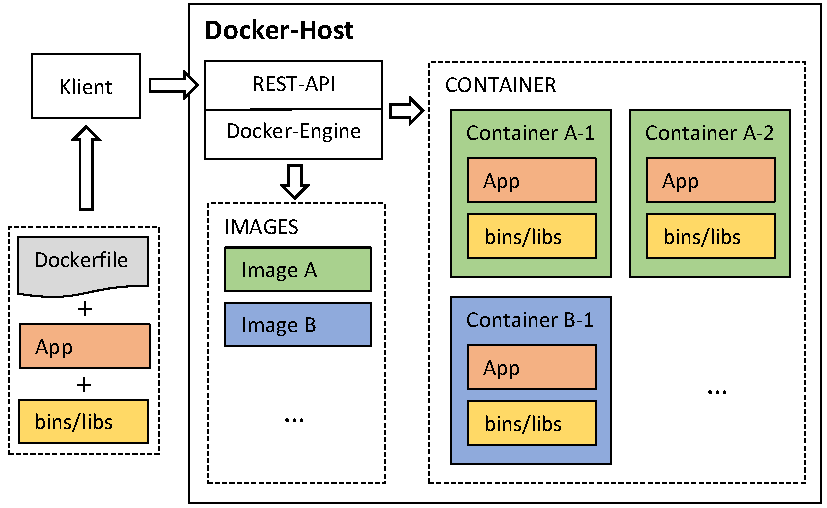
\includegraphics[width=\columnwidth]{docker-arch.pdf}%
\caption{Docker-Architektur}%
\label{fig:docker-arch}%
\end{figure}

Die genaue technische Umsetzung der Virtualisierung ist für des Betriebssystem spezifisch und übersteigt den Rahmen dieser Arbeit. Der folgende Abschnitt beschreibt nur einen komprimierten Überblick über einige grundlegende Konzepte im Betriebssystem Linux.

\subsection{Voraussetzungen für Betriebssystemvirtualisierung}
\label{subsec:docker-tech}

Ein Container ist nur auf der Betriebssystemebene von anderen Containern isoliert. Im Prinzip sind die in einem Container gestarteten Anwendungen  gewöhnliche Betriebssystemprozesse im Wirtsystem. Dennoch ist ein Container mehr ein virtuelles Betriebssystem als ein einfacher Prozess.

Die nachfolgenden Abschnitte basieren auf \cite{Merkel:2014:DLL:2600239.2600241}, sowie \cite{DBLP:journals/corr/Bui15} und beschreiben einige Betriebssystemkomponenten, die für die Virtualisierung verantwortlich sind.

\subsubsection{Namensräume}

\textit{Namensräume} bezeichnen im Betriebssystem \textit{Linux} eine Technologie, mit der Betriebssystemressourcen gruppiert und somit voneinander isoliert werden können. Dazu zählen beispielsweise Prozesse, Netzwerkverbindungen, das Dateisystem, \usw Diese Technologie stellt somit die Isolation zwischen Containern und auch zum Wirtsystem sicher.

\subsubsection{Kontrollgruppen}

Wie Abschnitt \ref{sec:isolation-vs-efficiencys} schon dargestellt hat, ist eine faire Ressourcenaufteilung zwischen Containern sehr wichtig. Linux bietet dafür das Konzept der Kontrollgruppen. Damit kann der Ressourcenverbrauch von Containern überwacht und gegebenenfalls deren Verbrauch limitiert werden.

\subsubsection{Überlagerte Dateisysteme}

Durch die Verwendung eines speziellen Dateisystems, kann Docker viele Daten zwischen Containern teilen und somit den Speicherplatz stark reduzieren. Die Grundidee ist, ein mehrschichtiges Dateisystem in eine einzige logische Sicht zu vereinen. Nur die oberste Schicht ist veränderbar. Alle anderen sind nicht beschreibbar und folglich unveränderbar. Eine Dateiänderung in einer höheren Schicht überdeckt die gleiche Datei einer niedrigeren Schicht.

Für beliebig viele Containerinstanzen ist somit nur eine einzige Kopie ihres Images auf der Festplatte notwendig. Mit dieser Technik ist eine enorme Speicherersparnis möglich, ohne die Isolation zu kompromittieren. Ein Betriebssystemabbild einer virtuellen Maschine mit Hardwarevirtualisierung ist um ein vielfaches größer und muss mehrfach abgespeichert werden. Je nach Betriebssystem gibt es verschiedene Implementierungen von überlagerten Dateisystemen. Zwei der bekanntesten Implementierungen sind das \textit{Advanced Multi-Layered Unification File\-system} und das \textit{OverlayFS}.

\subsection{Docker Beispiel}

Programm~\ref{prog:dockerfile} zeigt ein Beispiel für ein "`Dockerfile"', dass ein Image mit einem Web"=Service erstellt. Im Basis"=Image ist bereits .NET Core -- eine Abhängigkeit des Web"=Services -- vorinstalliert. Im Prinzip erhält die Beschreibung alle notwendigen Schritte, um den Web"=Service auf einem leeren System zu installieren und zu konfigurieren. Die in Programm~\ref{prog:dockercommands} angeführten Kommandozeilenbefehle, erzeugen aus der Imagebeschreibung aus Programm~\ref{prog:dockerfile} zuerst ein ausführbares Image und startet dieses anschließend.


\begin{program}[!hbt]
\caption{Beispiel für ein Dockerfile}
\label{prog:dockerfile}
\begin{DockerCode}
FROM microsoft/dotnet:1.1.1-runtime
COPY published app
WORKDIR app
ENV ASPNETCORE_URLS http://+:80 
EXPOSE 80
ENTRYPOINT [ "dotnet", "mywebapi.dll" ]
\end{DockerCode}
\end{program}

\begin{program}[!hbt]
\caption{Docker Kommandozeilenbefehle}
\label{prog:dockercommands}
\begin{GenericCode}
docker build -t sample-image .
docker run -d --rm -p 5000:80 sample-image
\end{GenericCode}
\end{program}

\section{Microsoft Windows Container}

Lange Zeit war Containervirtualisierung dem Betriebssystem Linux vorbehalten. Erst seit 2016 gibt es ein Äquivalent für Windows Betriebssysteme \cite{WinSerCont}. \textit{Windows Server 2016} ist das erste Windows Betriebssystem mit nativer Unterstützung für Containervirtualisierung auf Basis von \textit{Docker}. Auf fast allen Servern kommt entweder das Betriebssystem Linux oder Windows zum Einsatz. Dadurch die Möglichkeiten \textit{Docker} einzusetzen sehr groß. Sowohl Linux- als auch Windows-Systeme halten sich an die selben Schnittstellen von \textit{Docker}. Entwickler die mit einem System vertraut sind, können ihr vorhandenes Wissen auch auf der anderen Plattform wiederverwenden.

In Linux sind Container, wie in Abschnitt~\ref{subsec:docker-tech} beschrieben, über Namensräume voneinander isoliert. Windows verwendet den selben Ansatz, jedoch gibt es eine weitere Variante, die eine strengere Isolierung ermöglicht. Bei den sogenannten Hyper-V-Containern, läuft jeder Container in einer eigenen leichtgewichtigen und für Container optimierten Hyper-V virtuellen Maschine \cite{WinConHyperV}. Der Verwender kann somit sehr leicht zwischen Effizienz und Isolation wählen.

Jedes Image basiert auf einem anderen Image. Nur sogenannte Basis-Images besitzen kein Eltern-Image. Diese sind also die Basis für andere Images. Im Prinzip sind Images leere und auf ein Minimum reduzierte Standardbetriebssysteme. Aufgrund der vielen verschiedenen Distributionen gibt es für Linux"=Container sehr viele Basis-Images. Für Windows-Container hingegen gibt es nur zwei. Das sogenannte Windows"=Server"=Core"=Image ist im Prinzip eine vollständige Windows Server 2016 Installation, jedoch ohne Benutzeroberfläche. Es bietet viele Möglichkeiten, aber ist deswegen auch sehr groß. Eine schlankere alternative ist das Nano"=Server"=Image. Diese abgespeckte Variante wurde speziell für Container entwickelt. Tabelle \ref{tab:docker-image-size} zeigt den Speicherverbrauch von einigen ausgewählten Images und unterstreicht dabei die Leichtgewichtigkeit von Containern. Aufgrund der Wiederverwendbarkeit durch die geschachtelten Dateisystem ist der Speicherbedarf aber nicht so problematisch wie bei virtuellen Maschinen.

\begin{table}[!hbt]
\caption{Image-Größe von ausgewählten Basis-Images (März 2017)}
\label{tab:docker-image-size}
\centering
\setlength{\tabcolsep}{5mm} % separator between columns
\def\arraystretch{1.25} % vertical stretch factor
\begin{tabular}{|r||c|c|c|}
\hline
\emph{Image} & \emph{Plattform} & \emph{Größe (entpackt)} \\
\hline
\hline
Ubuntu & Linux & 128 MB \\
\hline
Debian & Linux & 123 MB \\
\hline
CentOS & Linux & 193 MB \\
\hline
Alpine & Linux & 4 MB \\
\hline
Windows Server Core & Windows & 10.1 GB \\
\hline
Windows Nano Server & Windows & 1 GB \\
\hline
\end{tabular}
\end{table}

\section{Containerverwaltung}

Einen Container auf nur einem Server zu betreiben ist eine triviale Aufgaben, aber hunderte Container auf einem Cluster mit mehreren Servern, ist ein ungleich komplexeres Unterfangen \cite{RussinovicContainers}. Aber dieses Szenario ist in einer Microservice"=Architektur eher die Regel als die Ausnahme. Um diese Herausforderungen zu bewältigen, wurden eine viele Werkzeuge für die Cluster- und Containerverwaltung entwickelt. Eine wichtige Funktion von diesen Werkzeugen ist es mehrere Container zu einer logischen Einheit zusammenzuschließen, sodass diese auch als Einheit verwaltet werden können. Des weiteren bieten diese Werkzeuge eine Abstraktion der tatsächlichen Infrastruktur. So können mehrere Server zu einem Cluster verbunden und dieser als kohärente Plattform betrachtet werden. 

Der Begriff Orchestrierung beschreibt in der Softwareentwicklung die Kombination mehrere Dienste zu einer Komposition. Auch bei Containern spricht man von Containerorchestrierung, wenn mehrere Container zu einer Einheit zusammengeschlossen werden um ihren Lebenszyklus gemeinsam zu verwalten. Ein Orchestrierer wird von vielen anderen Funktionen, wie \zB einem Scheduler oder einem Ressourcenmonitor unterstützt. 

Die Technologielandschaft rund um Containerverwaltung ist sehr breit und befindet sich noch stark im Aufbau. Eine umfassende Betrachtung dieses große Bereichs würde das Ausmaß dieser Arbeit übersteigen. Dennoch ist es für eine Arbeit wie diese, die sich mit dem Thema Microservices auseinandersetzt, unumgänglich diesen wichtigen Teilbereich zu erwähnen. Daher werden nachfolgend zumindest einige grundlegende Aspekte von Containerorchestrierung im Bezug auf Microservices dargestellt, die sich hauptsächlich auf \cite{ContainerOrcaWars} beziehen. 

\subsection{Funktionalität}

Die Hauptaufgaben eines Containerorchestrierers sind Maschinenbelegungsplanung, Ressourcen- und Serviceverwaltung. All diese Funktionen ermöglichen eine Reihe nicht"=funktionaler Eigenschaften wie Skalierbarkeit, Verfügbarkeit oder Portabilität von Containern. Die einzelnen Produkt am Markt unterscheiden vom Funktionsumfang und der Umsetzung der einzelnen Funktion.

\subsubsection{Maschinenbelegungsplanung}

Ein Orchestrierungswerkzeug muss entscheiden auf welchem Server eine oder mehrere Instanzen eines Containers erzeugt werden. Serverausfälle sollen automatisch erkannt und betroffene Container auf einem anderen Server neu gestartet werden. In manchen Fällen bieten sie auch eine Unterstützung bei der Aktualisierung von Containerversionen.

\subsubsection{Ressourcenverwaltung}

Alle Hardwareressourcen die ein Container in Anspruch nehmen kann, müssen überwacht und limitiert werden. Grundsätzlich betrifft das den Prozessor und den Hauptspeicher, aber auch persistenten Speicher und Netzwerkressourcen.

\subsubsection{Serviceverwaltung}

Mehrere Container werden zu einer einzelnen Applikation zusammengefasst, um sie gemeinsam zu verwalten. Im Zuge dessen müssen auch Abhängigkeiten zwischen Containern berücksichtigt werden, um beispielsweise eine sinnvolle Startreihenfolge festzulegen. Damit schlussendlich eine Anwendung auch skalierbar und hoch verfügbar ist, sind Lastverteilungsmechanismen notwendig, die auch vom Orchestrierungswerkzeug verwaltet werden.

\subsection{Verteilte Betriebssysteme}

Ein Betriebssystem bietet Anwendungsprogrammen eine Schnittstelle zu den Systemressourcen eines Computers. Somit müssen sich Anwendungsprogramme nicht mit der tatsächlichen Interaktion mit einer konkreten Hardwarekomponente auseinandersetzten, sondern sie greifen auf die abstrakten Schnittstellen des Betriebssystems zurück. Auch Containerorchestrierungswerkzeuge können als eine Art Betriebssystem verstanden werden, jedoch in verteilter Form. Statt Anwendungsprogramme teilt ein Orchestrierungswerkzeug Container \bzw aus vielen Containern zusammengesetzte Anwendungen, auf einen mit einer Containervirtualisierungssoftware ausgestatteten Rechner zu. Der Kern dieses Systems ist die Containervirtualisierungssoftware, die auf jedem der verteilten Rechner läuft und natürlich die Orchestrierungssoftware mit den im vorherigen Abschnitt beschriebenen Funktionen. Die verteilten Rechner und ihr tatsächliches Host"=Betriebssystem stellen die Systemressourcen dar. In vielen Fällen werden auch diese Systemressourcen als virtuelle Rechner zur Verfügung gestellt. In Abbildung~\ref{fig:container-distributed-os} ist die Analogie zwischen Betriebssystemen und Containerorchestrierungswerkzeugen noch einmal dargestellt.

\begin{figure}[!hbt]%
\centering
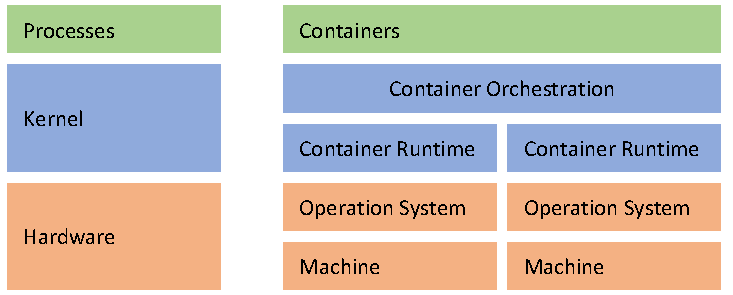
\includegraphics[width=.6\columnwidth]{container-distributed-os}%
\caption{Vergleich eines Betriebssystems (links) und eines "`verteilten Betriebssystems"' durch Containerorchestrierung}%
\label{fig:container-distributed-os}%
\end{figure}

\subsection{Marktanalyse}

Studien wie \cite{ContainerMarketGrowth} sehen Container mit einer geschätzten jährlichen Wachstumsrate von bis zu 40 Prozent bis 2020, als einen der größten Zukunftsmärkte im Bereich Cloud"=Computing. Aufgrund dieser Zahlen ist es auch nicht verwunderlich, dass in diesem Bereich sehr viel investiert wird und dementsprechend viele Produkte auf den Markt kommen. 

Laut \cite{ContainerMarketReport} ist \textit{Docker} mit 94 Prozent in 2016 das meist verwendete System für Containervirtualisierung. Jedoch bei der Containerorchestrierung sieht selbige Studie derzeit einen ausgeglichenere Markaufteilung zwischen den Produkten \textit{Docker Swarm}, \textit{Kubernetes} und \textit{Apache Mesos}, wobei \textit{Kubernetes} die meisten Anteile dazugewinnen konnte.

\section{Zusammenfassung}

In diesem Kapitel wurde Containervirtualisierung, im speziellen mit \textit{Docker}, als mögliche Plattform für Microservices vorgestellt. Ähnlich wie mit virtuellen Maschinen ist es mit \textit{Docker} möglich eine Anwendung mit allen Abhängigkeiten zu verpacken, zu verteilen und zu betreiben. Jedoch ist Containervirtualisierung viel effizienter und benötigt weniger Speicherplatz als Hardwarevirtualisierung.

Anstatt einer langlebigen Server"=Infrastruktur deren Software und Konfiguration laufend Aktualisiert wird, setzt man heutzutage eher auf eine unveränderbare Infrastruktur. Das heißt anstatt einen Server zu aktualisieren wird er durch einen neuen ersetzt. Virtualisierungsplattformen wie \textit{Docker} haben diesen Ansatz extrem effizient und robust gemacht.

Container alleine decken aber längst nicht alle Anforderungen an einen Infrastruktur für Microservices ab. Schnell sind Funktionen für die Skalierung, Verteilung, Aktualisierung oder die Überwachung von Containern notwendig. Für diese Aufgabe gibt es eine Menge von Containerorchestrierungswerkzeugen, die als eine Art verteiltes Betriebssystem über der Containervirtualisierung agieren.

Unumstritten sind Container eines der zukunftsträchtigsten Technologiefelder der letzten Jahre, getrieben durch die DevOps"=Kultur und die Microservices"=Architektur. Vor allem im Bereich von Cloud"=Computing haben sie sehr großes Potential. Die Zukunft wird zeigen, ob und wie sich Container zwischen allen bestehenden \textit{Plattform-as-a-Service} Angeboten platzieren können. 